\title{Analysis~and~reproducibility~of~paper ``A~Word~Embedding~based Generalized~Language~Model for~Information~Retrieval'', D.~Ganguly,~D.~Roy,~M.~Mitra,~G.J.F. Jones,~2015.}

\author{Alessio~Lazzaron,~Matteo~Marchiori,~Andrea~Oriolo,~Fabio~Piras,~\IEEEmembership{Group~IR1.3}}

\maketitle

\IEEEraisesectionheading{\section{Introduction and Comprehension}\label{sec:introduction}}
\IEEEPARstart{W}{ith} the term Statistical Language Modeling or more simply Language Modeling (LM), we mean the development of probabilistic models that are able to predict a term given a context.

Due to the ambiguity of human language and its intrinsic properties, this process is very difficult to reproduce; however, several models have been developed over the years in order to estimate word representations. Some examples are: Latent Semantic Analysis (LSA), where the terms are represented in a space of reduced dimensionality; Latent Dirichlet Allocation (LDA), which goes to represent the dependencies of the terms assuming that each of them is generated by a set of latent variables called topics.

The main problem is that these models care only about  the occurrences of words at the level of individual documents, leading to results that are not always very reliable.
In this paper the Generalized Language Model (GLM) is proposed \cite{paper:ganguly}, an information retrieval model that allows you to directly model the dependencies of a term using the Word Embedding technique, thus allowing you to store both semantic and syntactic information of words in a space vector. The closer the vectors are the more the words are semantically similar, that is, they occur in the same linguistic contexts.

Unlike the basic Language Model, which assumes that each term is independent from each other, the Word Embedding technique takes into consideration the local context of the word in order to create a better model for predicting the dependencies among terms and thus significantly improving the quality of the retrieval.
With the Generalized Language Model we want to generalize the basic Language Model paradigm by transforming a term ${t}'$ of a document into a term $t$ of the query through a noise channel.

In detail, this transformation process can take place in 3 ways:
\begin{itemize}
    \item Direct term sampling: no transformation takes place, it represents the standard Language Model;
    \item Transformation via document sampling: the term $t$ is generated starting from a term ${t}'$ belonging to the document;
    \item Transformation via collection sampling: the term $t$ is generated starting from a term ${t}'$ belonging to the collection.
\end{itemize}

Once the terms have been calculated using these three approaches, the generalized model involves the combined use of all three methodologies.
The following figure shows how is it possible to build the model:

\begin{figure}[htp]
    \centering
    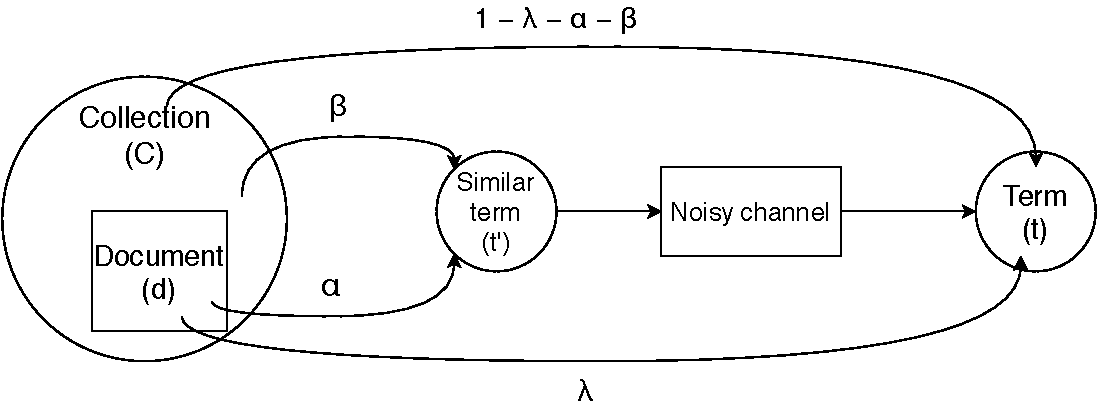
\includegraphics[width=\columnwidth]{glm}
    \caption[Generalized Language Model]{Schematics of generating a query term $t$ in our proposed Generalized Language Model (GLM). GLM degenerates to LM when $ \alpha = \beta = 0$.}
    \label{fig:glm}
\end{figure}

From our point of view, this transformation process calculates a similarity value between the term ${t}'$ and $t$ or how semantically similar the two terms are in the representation of the Word Embedding.

According to the GLM, the probability of the query term $t$, given a document $d$ in collection $C$, is provided by the following equation:

\begin{equation}
    \begin{split}
    P(t|d) & = \lambda P(t|d)\\
    & + \alpha \sum_{{t}'\in d}P(t,{t}'|d)P({t}')\\
    & + \beta \sum_{{t}'\in N}P(t,{t}'|C)P({t}')\\
    & + (1-\lambda-\alpha-\beta)P(t|C)
    \end{split}
\end{equation}

\clearpage

In detail:
\begin{itemize}
    \item the first term in lambda represents the probability of observing a query term $t$ without the transformation process;
    \item the probability of observing a term $t$ obtained by transforming a term ${t}'$ sampled from the document is represented by the second term in alpha in the formula;
    \item the third term of the formula in beta represents the probability of observing the term $t$ obtained from the transformation of ${t}'$ from the entire collection;
    \item the last term represents the remaining probability of observing a term $t$ from the collection without the transformation process.
\end{itemize}

This model takes into account the correlation of terms using the transformations
mentioned above.

Analyzing in detail every single probability: 
    
\begin{equation}
    \lambda P(t|d)=\lambda \frac{tf(t,d)}{|d|}
\end{equation} is the probability of the term $t$ of the query within the document $d$, calculated as the frequency of the term with respect to the number of words in the document.
$\alpha$ is the weight assigned to the probability of transformation of the term $t$ into the term ${t}'$, with ${t}'$ belonging to the document $d$.

\begin{equation}
    \begin{split}
    &\sum_{{t}'\in d}P(t,{t}'|d)P({t}')=\\
    &\sum_{{t}'\in d}\frac{sim(t,{t}')}{\sum_{{t}''\in d}sim(t,{t}''))}\frac{tf({t}',d)}{|d|}P({t}')
    \end{split}
\end{equation}
is the sum of the probabilities of transforming the term $t$ of the query into a term ${t}'$ of the document $d$.

$\beta$ is the weight assigned to the probability of transforming the term $t$ into the term ${t}'$, with ${t}'$ belonging to the collection $C$.

\begin{equation}
    \begin{split}
        & \sum_{{t}'\in Nt}P(t,{t}'|C)P({t}')=\\
        & \sum_{{t}'\in Nt}\frac{sim(t,{t}')}{\sum_{{t}''\in Nt}sim(t,{t}''))}\frac{cf({t}')}{cs}P({t}')
    \end{split}
\end{equation}
is the sum of the probabilities of transforming the term $t$ of the query into a term ${t}'$ belonging to the collection $C$.

\begin{equation}
    \begin{split}
        & (1-\lambda-\alpha-\beta)P(t|C)=\\
        & (1-\lambda-\alpha-\beta)\frac{cf(t)}{cs}
    \end{split}
\end{equation}
is the probability of the term $t$ of the query to be inside the collection $C$.


The Cosine similarity is used to calculate similarity, a technique used to measure the similarity of two terms through the cosine of the angle between the vectorial representations of the two.
In detail, given two vectors A and B, which respectively represent the terms $t$ and ${t}'$, the score of similarity can be calculated as follows:
\begin{equation}
    \begin{split}
        sim(A,B) & =\cos(\theta)=\frac{A*B}{||A||||B||}\\
                 & =\frac{\sum_{i=1}^{n}Ai*Bi}{\sqrt{\sum_{i=1}^{n}Ai^{2}}*{\sqrt{\sum_{i=1}^{n}Bi^{2}}}}
    \end{split}
\end{equation}
The peculiarity, in our case, lies in the fact that the vectors are represented in the form of embedding.
Among the existing techniques, Word2Vec was used for creating the embedding of words.
This methodology, based on the use of neural networks, allows you to obtain predictions about words, assign a probability distribution to terms and also allows you to better capture analogies and similarities between semantically related words.
In this case Word2Vec is used to extract the embeddings of the terms or their vectorial representation, leaving out the tasks of the respective neural networks.

Taken each term ${t}'$ from the collection or document, we calculate the similarity between these and the term $t$ of the query.
As the similarity value increases between a term $t$ of the query and the terms ${t}'$ of the document and the frequency of each similar ${t}'$ within the document, the value of the second term (\(\alpha\)) in Formula 1 also increases.
This means that the terms inside of the document are semantically similar to the term $t$ of the query and therefore the term $t$ fits well with the document.
If, at the same time, the similarity between the term of the query $t$ and the terms ${t}'$ taken from the collection is high, the third term of Formula 1 will be higher. To avoid taking all the terms in the collection, a list of neighbors of the word is precalculated in order to make the calculation more efficient.
This model favors documents containing terms that are semantically similar to the query term $t$.
In fact, semantically similar words tend to contribute more to the increase in the score of the term $t$, which will better adapt to the context of a document with terms closer to it. The higher the similarity value, the more relevant the correspondence between the terms will be.
